\documentclass[conference]{IEEEtran}
\usepackage{graphicx}
\usepackage{cite}
\usepackage{url}
\usepackage[cmex10]{amsmath}
\usepackage{algorithmic}
\usepackage{array}
\usepackage{mdwmath}
\usepackage{mdwtab}
\usepackage{eqparbox}
\usepackage[font=footnotesize]{subfig}
\usepackage{fixltx2e}
\usepackage{setspace}
\usepackage[ruled,vlined,commentsnumbered]{algorithm2e}
\usepackage{amssymb}
\usepackage{amsthm}

\newtheorem{thm}{Theorem}


\begin{document}

\title{A Distributed Algorithm for Minimizing Travel Time in Traffic Grids}

\author{\IEEEauthorblockN{Chinwei ``Vic'' Hu}
\IEEEauthorblockA{Department of Electrical and Computer Engineering}
\IEEEauthorblockA{The University of Texas at Austin}
\IEEEauthorblockA{vic@cvhu.org}
\and
\IEEEauthorblockN{Saddam Quirrem}
\IEEEauthorblockA{Department of Electrical and Computer Engineering}
\IEEEauthorblockA{The University of Texas at Austin}
\IEEEauthorblockA{s\_quirrem@hotmail.com}
}
\maketitle
\onehalfspace
\begin{abstract}
Modern traffic control systems often loop through a set of basic states, with little or no regard to the real-time traffic conditions and communications with neighboring systems. In this paper, we proposed a distributed algorithm, LAWQS, to design a communicative network of traffic management systems that are self-adaptive to real-time incoming traffic. We implemented a simulation framework to compare our algorithm against the traditional traffic light protocol, and was able to show a promising improvements in both vehicle traveling times and intersection traffic loads.
\end{abstract}

\section{Introdution}

The average commute time in the United States is 25.4 minutes \cite{commuting_time}, and 80\% of workers drive to work everyday. In 2011 along, American drivers spend 5.5 billion productive hours sitting in the traffic, costing the nation \$121 billion dollars \cite{commuting_expense}. 

Our current traffic infrastructure has been used for over a century, which wasn?t designed for the amount of traffic in the modern society. Most of the traffic lights and stop signs on the intersections today still use an inadaptable and synchronous architecture that waste a ton of unused time and space on the roads. Looking at the core concepts developed in communication networks, computer architecture, and distributed computing, many technologies such as virtual memory, pipelining, and network routing, are trying to solve very similar problems we are facing on the roads everyday. By introducing a few straightforward but yet powerful concepts, we wish to expand academia interests to solve these persisting problems in our current traffic control system.

In this paper, we introduced a simulation framework to model and simplify the sophisticated traffic systems, a set of measuring criteria to make quantitative analysis, a benchmark DUMMY algorithm, a Look-Ahead algorithm, a WeightedQ-Switcher algorithm, and a combination of these two algorithms. The rest of this paper is organized as following: section 2 covers the basic backgrounds, terminology, and notations; section 3 introduces the main algorithms; section 4 presents the experiment results, comparison analysis and discussions on our algorithms; section 5 makes the conclusion.


\section{Background}
In this section, we will cover how the sophisticated traffic systems with a large degrees of uncertainty can be simplified and represented in a GridWorld model. Furthermore, we will formalize the problem we are trying to solve, go over some intuitions behind our solutions, and make clear definitions about the notations we will be using.

\subsection{The GridWorld Model}
There are a great variation of possible configurations and protocols used in the real-world traffic systems. In our study, we only consider a two-lane, four-way configuration with all intersections perfectly aligned in a m-by-n GridWorld, as shown in Fig.~\ref{gridworld_barebone}

\begin{figure}[h]
    \center    
    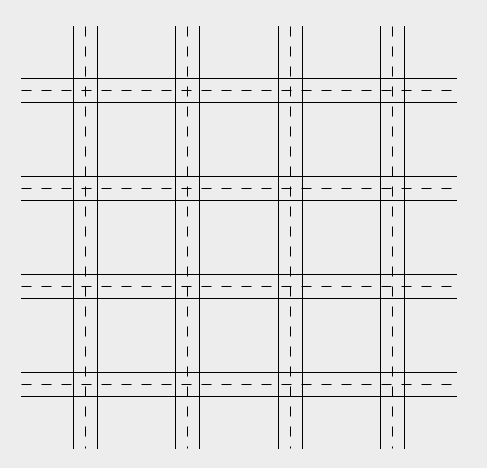
\includegraphics[width=0.25\textwidth]{images/gridworld_barebone.png}
	\caption{a 4-by-4 GridWorld model}
	\label{gridworld_barebone}
\end{figure}


The intersections are modeled as a distributed system organized on a grid. We assume that each incoming vehicle is equipped with a communicating device such as a smartphone or a BlueTooth beacon, that is able to send requests to the upcoming intersection, and notify the driver when requests are granted. We also assume that there is an application server installed at each intersection on the grid, which can communicate with its neighboring peers and respond to vehicles that have sent requests to it.

For instance, intersection at (0,0) refers to the southwestern corner of the grid, and intersection (n-1,m-1) refers to the northeastern corner of the grid. Each intersection acts as an independent node and has a direct two-way communication channel with its four neighboring intersections. This means intersection (x,y) can send and receive messages from intersections (x-1,y), (x+1,y), (x,y-1), and (x,y+1) if they exist in the grid. Each intersection server maintains four queues of vehicles (clients), and allows the head of each of these queues to pass if its requested direction matches the current state of the intersection server. The clients themselves perform two simple task. First they send a request to the facing intersection and wait until their request is acknowledge by an intersection server. When acknowledged, the vehicle client moves on to the next intersection, and continues until it reaches its destination.

\subsection{The Intersection/Vehicle Architecture}
Each intersection server is essentially a finite state machine consisting of four states: \texttt{VERTICAL\_STRAIGHT}, \texttt{VERTICAL\_LEFT}, \texttt{HORIZONTAL\_STRAIGHT}, and \texttt{HORIZONTAL\_LEFT}, as shown in FIg.~\ref{intersection_states} \texttt{VERTICAL\_*} states handle requests coming from the north and south directions, while \texttt{HORIZONTAL\_*} states handle those from west and east. A request going straight and right is granted at \texttt{*\_STRAIGHT} states, while a left-turn request are granted at \texttt{*\_LEFT} states.

\begin{figure}[h]
    \center    
    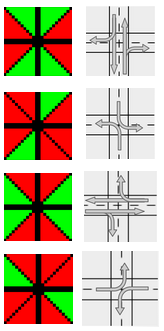
\includegraphics[width=0.25\textwidth]{images/intersection_states.png}
	\caption{the four intersection states}
	\label{intersection_states}
\end{figure}

Each vehicle is assigned with a final destination and starting position, both of which are represented as an intersection on the grid. At each intersection, a vehicle can either take left, right, or go straight. There are two different kinds of vehicles. Ones that have a predetermined route to take, and ones that only specify the final destination and don?t care about the path. Note that the former can be easily mapped as a sequence of immediate short-term destinations, each spaced one block apart. Thus, the request protocol can be simply represented as the desired current destination node.

\subsection{Problem Definition and Requirements}
Now that we have a clearly defined framework and a simplified model of our system, let?s revisit the problem and the requirements we are trying to achieve. In general, we want an algorithm that is distributed, scalable, flexible, adaptive, and secure; a system that can be reasonably integratable to our existing infrastructure. \\

\noindent  {\it \textbf{Problem Definition:} Given any grid configurations and vehicle routes, come up with a distributed algorithm to minimize time spent travelling and to even out intersection loads.}\\

In the real-world application, each vehicle ultimately only cares about how fast it can reach from the starting position to the final destination. In that regard, it?s obvious that everyone with the same destination is going to take the same optimal routes, creating high chance of gridlocks and leaving the rest of the grids unused. Therefore, we introduce a second objective function to even out the intersection loads to speed up the learning process.\\

\noindent {\bf Requirements:}
\begin{itemize}
\item {\bf Distributivity} To make the system architecture infinitely scalable, the algorithm should only communicate and utilize information of its own node and the neighboring nodes.
\item {\bf Safety} No conflicting traffic should be granted access to the intersection at anytime, any node.
\item {\bf Liveness} All requests should be granted within finite time.
\item {\bf Fairness} First come, first serve.
\end{itemize}
\-\\
Similar to traditional distributed algorithms, these four fundamental requirements will be used to examine the correctness of our algorithms in the next section.


\section{Algorithms}
In this section, we introduce four algorithms to be tested in our simulation framework: Dummy, Look-Ahead (LA), WeightedQ-Switcher (WQS), and LA-WQS.

\subsection{Intuitions}
The Dummy algorithm represents the benchmark, which resembles the conventional traffic lights we see everyday on the street. It loops through a set of predefined states regardless of the real-time traffic. We use it as the baseline algorithm to demonstrate the effectiveness of our proposed ones.
The Look-Ahead (LA) algorithm makes suggestions to incoming vehicles on the optimal action based on its neighborhood conditions. The vehicle only sends its desired final destination; the intersection server evaluates all the candidate immediate actions and responds to the request with the suggested action.

The WeightedQ-Switcher (WQS) algorithm makes decisions on state transition based on the weights of request queues. Each request sitting in the queue keeps a counter to represent how long it?s been waiting, and the sum of those counter values in a queue is the weight. When the intersection finishes a state operation, it picks the next state with the largest sum of weights.

Finally, the LA-WQS algorithm is simply a combination of both LA and WQS.

\subsection{ Algorithms for Vehicles}
There are two different kinds of vehicles: a PathVehicle that predetermines the route to take, and a DestVehicle that only specify the final destinations. 

As shown in Algorithm.~\ref{path_vehicle}, the vehicle simply sends a request to the intersection server for each move, and waits until the request is granted by the server. When the request is granted, the server process calls the \texttt{receiveRequestOkay(nextPos)} function of the vehicle with the suggested next move, in which the vehicle moves on and continues the traversing procedure.

\begin{algorithm}
  \KwData{Start position and final destination}
  \KwResult{Computes the destinationQueue and traverses through the path.}
  init destQ = generatePath(start, finalDest)\;
  init currentPos = start\;
  init currentDest = destQ.pop()\;
  \While{currentDest != null}{
  	sendRequest(currentPos)\;
	wait()\;
  }
  
\SetKwFunction{receiveRequestOkay}{receiveRequestOkay}
\SetKwProg{myproc}{Function}{}{}

\myproc{\receiveRequestOkay{nextPos}}{
  	Moves the vehicle to nextPos\;
	\If{currentDest == currentPos}{
		\If{destQ is not empty}{
			currentDest = destQ.pop()\;
		}
		\Else{
			currentDest = null\;
		}
	}
	notify()\;
 }

  
\SetKwFunction{generatePath}{generatePath}

\myproc{\generatePath{start, finalDest}}{
  init destQueue\;
  currentPos = start\;
  \While{currentPos != finalDestination}{
  	currentPos = randomWalk(currentPos, finalDest)\;
	destQueue.push(currentPos)\;
  }
  \KwRet destQueue\;
 }
  \caption{PathVehicle \label{path_vehicle}}
\end{algorithm}

The DestVehicle employs a very similar model, except that there is no \texttt{generatePath} procedure anymore and \texttt{destQ} only contains the final destination.


\subsection{ Algorithms for Intersections}

Now we've covered the behavior of vehicle clients, let's look at algorithms followed by the server process at each intersection.

\subsubsection{ Dummy Algorithm}

The Dummy algorithm is what we used as the baseline benchmark to measure the effectiveness of our proposed algorithms. It resembles the traditional traffic light system that loops through a predetermined set of states and durations, regardless of the real-time traffic conditions. As mentioned in Fig.~\ref{intersection_states}, we modeled the traffic light system into a static finite state machine, consisting of \texttt{VERTICAL\_STRAIGHT}, \texttt{VERTICAL\_LEFT}, \texttt{HORIZONTAL\_STRAIGHT}, and \texttt{HORIZONTAL\_LEFT}. The state machine for the Dummy algorithm is illustrated in Fig.~\ref{dummy_state}.

When a vehicle sends requests to an intersection, the server puts it into one of the four queues it keeps for each traffic direction: \texttt{north}, \texttt{south}, \texttt{easy}, and \texttt{west}. At each state, the server examines the legal conditions of frontiers at the associated queues, and grants the requests if validated.

\begin{figure}[h]
    \center    
    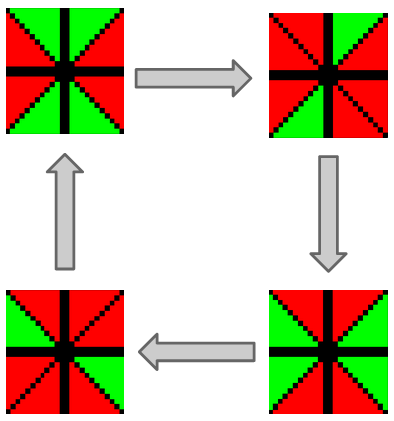
\includegraphics[width=0.25\textwidth]{images/dummy_state.png}
	\caption{a finite state machine for the Dummy algorithm}
	\label{dummy_state}
\end{figure}

\begin{figure}[h]
    \center    
    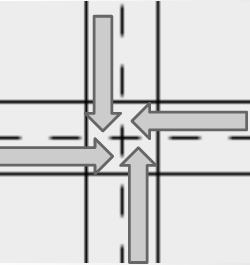
\includegraphics[width=0.2\textwidth]{images/direction.png}
	\caption{Each intersection server keeps a queue to store requests coming from each direction.}
	\label{direction}
\end{figure}


\begin{algorithm}
  \KwData{Four requestQueues for each traffic direction.}
  \KwResult{Grants requests based on the current state.}
  init requestsQMap as a hash map of request queues with direction as keys\;
  init FSM as the finite state machine defined in Fig.~\ref{dummy_state}\;
  \While{running} {
  	currentState = getState(FSM)\;
	\For{requestsQ in legal queues of currentState}{
		frontRequest = requestsQ.peek()\;
		\If{frontRequest is legal}{
			grant frontRequest \;
			requestsQ.pop()\;
		}
	}
  }
  \caption{Dummy \label{dummy}}
\end{algorithm}

  The legal states mentioned in Algorithm.~\ref{path_vehicle} are determined according to the current state: requests queues of north and south are used when at \texttt{VERTICAL} states, while queues of east and west are used at \texttt{HORIZONTAL} states.

\subsubsection{ Look-Ahead (LA) Algorithm}

Instead of granting incoming requests with a fixed path specified by the vehicle, the Look-Ahead algorithm makes suggestions on the optimal action based on the real-time traffic conditions of neighboring intersections. 

In Fig.~\ref{la_example}, a vehicle from the bottom right intersection is trying to reach the top left destination. Normally, an instance of PathVehicle has no prior knowledge on the traffic conditions, so it chooses both north and east with equal probability in a random walk path generating procedure. The Look-Ahead algorithm, on the other hand, sends messages to its neighboring intersection processes to get the queue sizes corresponding to the candidate actions, and suggests the vehicle to take the less-crowded route when granting the request.



\begin{figure}[h]
    \center    
    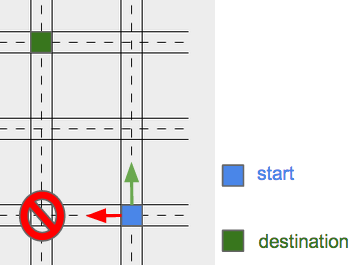
\includegraphics[width=0.25\textwidth]{images/la_example.png}
	\caption{Look-Ahead algorithm allows upcoming traffic to avoid neighboring gridlocks.}
	\label{la_example}
\end{figure}

\begin{algorithm}
  Everything is the same as in Algorithm.~\ref{dummy}, except that when granting a request, the server makes action recommendation based on the following procedure:
  
\SetKwFunction{getOptimalAction}{getOptimalAction}
\SetKwProg{myproc}{Function}{}{}
\myproc{\getOptimalAction{destination}}{
	init minSize = -$\infty$\;
	init actionOptimal = null\;
  	\For{action in candidateActions}{
		\If{queue size with action < minSize}{
			minSize = queue.size()\;
			actionOpt = action\;
		}
	}
	\KwRet actionOpt\;
 }
  \caption{Look-Ahead (LA) \label{look_ahead}}
\end{algorithm}

The concepts behind Look-Ahead is very similar to Dijkstra's shortest path \cite{dijkstra} with horizontal of size one, and is fairly simple to implement. For each request, there are one request message, two to four look-ahead messages, and one response message. In practice, the neighboring queue size data could be cached in the current intersection server, and updates could be accomplished by a publisher/subscriber paradigm. In such cases, the message complexity can be reduced down to size two, which is the same as in Dummy.

One of the biggest disadvantage in both Dummy and Look-Ahead is that they both utilizes static state transitions, which wastes a lot of unused cycles and resources as in most synchronous systems. Next, we will talk about how the WeightedQ-Switcher algorithm addresses exactly this problem.

\subsubsection{WeightedQ-Switcher (WQS) Algorithm}

In our analysis for the Dummy and Look-Ahead algorithms, we discussed how a hard-coded state machine suffers from wasted resources and computation cycles, which could be resolved by designing an adaptive system that makes state transition decisions based on the real-time traffic. In this section, we propose the WeightedQ-Switcher algorithm to give a simple example on how that could be done in practice.

As shown in Fig.~\ref{wqs_state}, the state machine presented in Fig.~\ref{dummy_state} is separated into a dynamic, two-state machine. The new \texttt{VERTICAL} state consists of both \texttt{VERTICAL\_STRAIGHT} and \texttt{VERTICAL\_LEFT}, which takes care of the traffic from north and south before either switching to \texttt{HORIZONTAL} or staying in \texttt{VERTICAL}, and similarly for the transitions in \texttt{HORIZONTAL}.

\begin{figure}[h]
    \center    
    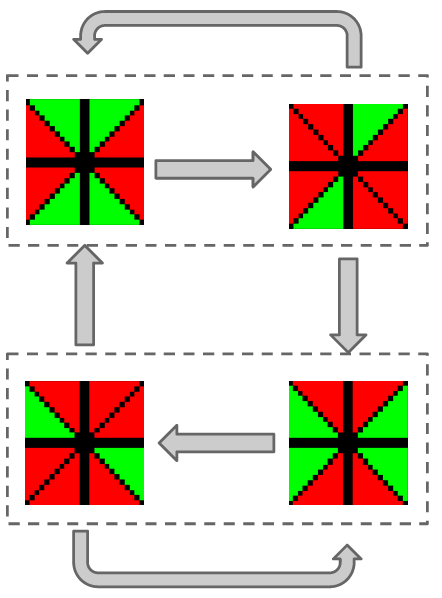
\includegraphics[width=0.25\textwidth]{images/wqs_state.png}
	\caption{A dynamic state machine of WQS}
	\label{wqs_state}
\end{figure}

In Fig.~\ref{wqs_decision}, we see how WQS decides which state to go next based on \texttt{w(VRTL)}, the weights of vertical queues, and \texttt{w(HRZL)}, the weights of horizontal queues. Note that if we naively define queue weights as the total number of requests, we may easily run into cases where requests sitting in certain queues are never processed, and hence suffer from starvation. Therefore, we incorporate a counter parameter for each waiting elements in queues, which represents how many rounds it's been waiting for the server process. 

\begin{figure}[h]
    \center    
    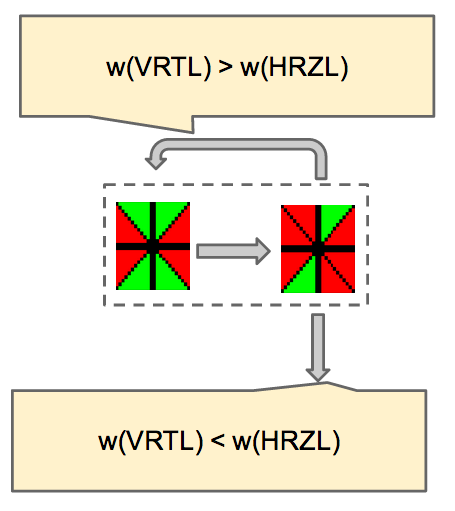
\includegraphics[width=0.3\textwidth]{images/wqs_decision.png}
	\caption{State transitions in WQS is now based on the queue weights.}
	\label{wqs_decision}
\end{figure}

More details on this procedure are specified in Algorithm.~\ref{wqs}, in which we omitted parts that are duplicated from previous algorithms.

\begin{algorithm}
  Everything is the same as in Algorithm.~\ref{dummy}, except that when transitioning to the next state, the intersection server calls the following procedure:
  
\SetKwFunction{getNextWQSState}{getNextWQSState}
\SetKwProg{myproc}{Function}{}{}
\myproc{\getNextWQSState{}}{
	init nextState = null\;
	init weightVertical = getWeight(north) + getWeight(south)\;
	init weightHorizontal = getWeight(east) + getWeight(west)\;
	\If{weightVertical > weightHorizontal}{
		nextState = VERTICAL\;
	}
	\ElseIf{weightVertical < weightHorizontal}{
		nextState = HORIZONTAL\;
	}
	\Else {
		nextState = random(VERTICAL, HORIZONTAL)\;
	}
	\KwRet nextState\;
 }
 
 \SetKwFunction{getWeight}{getWeight}
\SetKwProg{myproc}{Function}{}{}
\myproc{\getWeight{direction}}{
	init weight = 0\;
	\For{request in requestsQMap.get(direction}{
		weight += request.getCounter()\;
	}
	\KwRet weight\;
 }
 
  \caption{WeightedQ-Switcher (WQS) \label{wqs}}
\end{algorithm}

In the real-world analogy, we can think of WQS as a mean to allow queues that are large and have been waiting longer than others to pass with privilege. On the other hand, if there is no traffic on the other direction, one would never have to stop unnecessarily.


\subsubsection{ LA-WQS Algorithm}
As the name suggests, LA-WQS is a combination of both the afore-mentioned Look-Ahead and WeightedQ-Switcher algorithms.

\subsection{Correctness Analysis}

\begin{itemize}
\item {\bf Distributivity} All the presented algorithms satisfy this property, in that they can all be implemented in each intersection process in exactly the same way.
\item {\bf Safety} When processing the queue frontiers, the process always checks for legal moves corresponding to the current state. Hence, all algorithms preserver safety.
\item {\bf Liveness} Both Dummy and Look-Ahead would eventually grant every requests within finite time since they visit each queue with equal probability. Although their might be chance of starvation in a naive approach of WQS, we've presented a counter variable to guarantee long-waiting request to be granted even when the other queues are very long.
\item {\bf Fairness} This property can only be partially satisfied within each queue. However, requests arriving at the same time wouldn't vary for more than one full cycle.
\end{itemize}

\subsection{ Complexity Analysis}

\begin{table}[h]
	\center
	\begin{tabular}{ll p{4cm}}
	\hline
	Algorithm & Messages & Explanation\\
	\hline
	\hline
	Dummy & O(2N(W+H)) & Intersections do not communicate. One message from vehicle, one message back.\\
	\hline
	LA & O(6N(W+H)) & Intersection sends up two query messages per vehicle, plus one from vehicle, plus one back.\\
	\hline
	WQS & O(2N(W+H)) & Intersections do not communicate. One message from vehicle, one message back.\\
	\hline
	LA-WQS & O(6N(W+H)) & Similar to LA.\\
	\hline
	\end{tabular}
\end{table}

\section{Experiments}
\subsection{Testing Methodology}
The average velocity, measured as the number of nodes traveled divided by the time taken for a vehicle to reach its destination, is used to compare the performance of each algorithm. The algorithms will be tested with various grid size and the number of vehicles. A higher average velocity indicates a higher throughput.

\subsection{Results and Discussion}
The results show that making use of a distributed algorithm leads to a more even distribution of vehicles across the grid and greater throughput. Some basic runtime analysis was performed on four algorithms with grid sizes ranging from 4x4 to 8x8 and 256 or 512 vehicles, as shown in Fig.~\ref{simulation_duration}.

\begin{figure}[h]
    \center    
    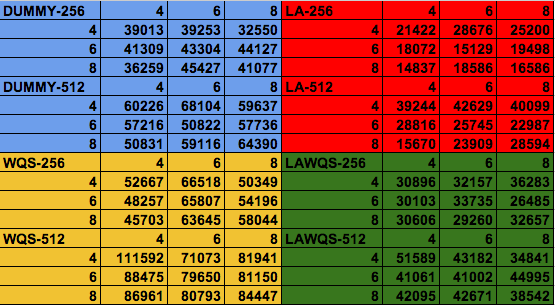
\includegraphics[width=0.45\textwidth]{images/simulation_duration.png}
	\caption{runtime analysis for various simulation configurations}
	\label{simulation_duration}
\end{figure}


These results cannot be used to evaluate the throughput based on the size of the grid, because much of the runtime is taken up by a few vehicles which have fallen behind, in addition to the unreliable nature of physical clocks. Nonetheless, what can be taken from these results is which algorithms  generally outperform the others. From these results, we can see that the top performing algorithms are ordered as Lookahead, LA-WQS, Dummy, and WeightedQ-Switcher. 

Contrary to what our initial hypothesis, switching states based on the {\it weights} of the lanes is not beneficial in our test cases. One explanation is that the intersection servers spend more time servicing only one lane, while the other three lanes eventually get clogged, namely starvation. This creates a cycle where the intersection server would keep serving heavier lanes of increasing weight until no more vehicles are coming in. One future improvement we can make based on this assumption, is to increment the counter exponentially to outweigh the penalty for starvation over queue lengths.

The combination of the lookahead algorithm and the weightedQ-switcher, LA-WQS, actually managed to outperform the dummy algorithm. This shows that just by adding a distributed algorithm to a slower non-distributed algorithm, we were able to outperform the simplest implementation. An analysis of the server workloads in Fig.~\ref{intersection_load} shows how traits of our WQS and LA algorithm were inherited by the LA-WQS algorithm.


\begin{figure}[h]
    \center    
    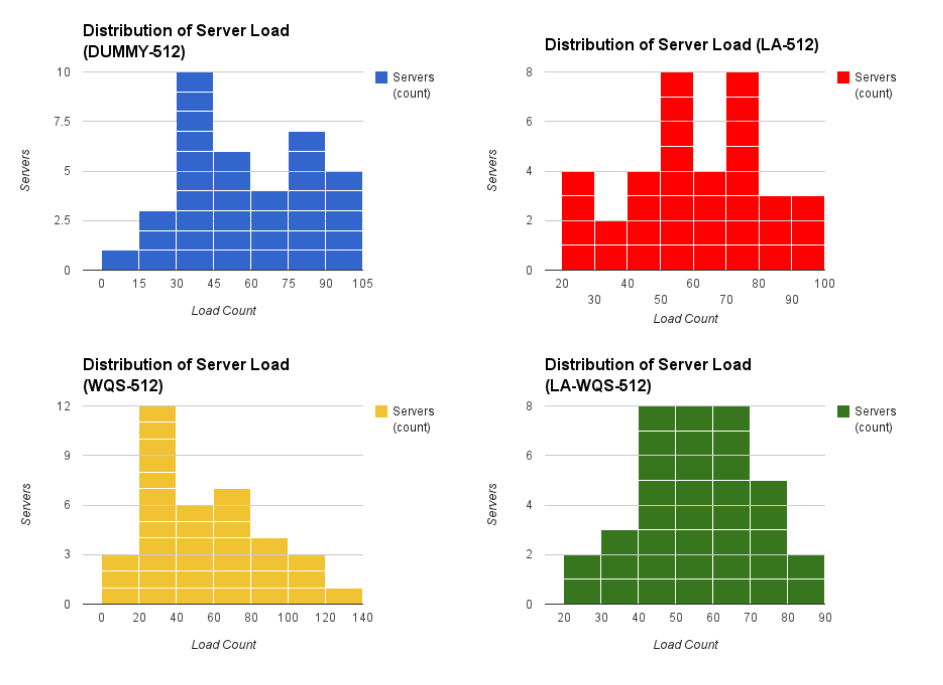
\includegraphics[width=0.5\textwidth]{images/intersection_load.png}
	\caption{histogram of server load distribution. from top-left, clockwise: DUMMY, LA, LA-WQS, WQS}
	\label{intersection_load}
\end{figure}


Diagrams in Fig.~\ref{intersection_load} are histograms displaying the number of servers in each workload bucket, where each bucket is identified by how many vehicles a server has processed during the simulation. An ideal algorithm would have a nice and evenly distributed loads across all available intersection servers, giving a normal distribution with low standard deviation. The Look-Ahead algorithm shows a somewhat normal distribution, which is inherited by the LA-WQS algorithm?s distribution. On the other hand, the Dummy algorithm tends to yield high server loads, skewing the load distribution to the higher end, while WQS effectively skews down the server loads for most intersections.

The motion of the vehicles provides the overall throughput of the system. The rate of motion is calculated as the average number of logical clock cycles it takes to move in one intersection-step. A lower number of logical clock cycles per move would be indicative of a higher throughput and less traveling time wasted. The four algorithms were tested using the same configurations to collect the server workload data as to extract the vehicle motion data.

In Fig.~\ref{vehicle_motion}, we can clearly observer that all LA, WQS, and LA-WQS skew the waiting time to the lower end and improve the overall throughput of the traffic, with LA providing the most significant improvements.

\begin{figure}[h]
    \center    
    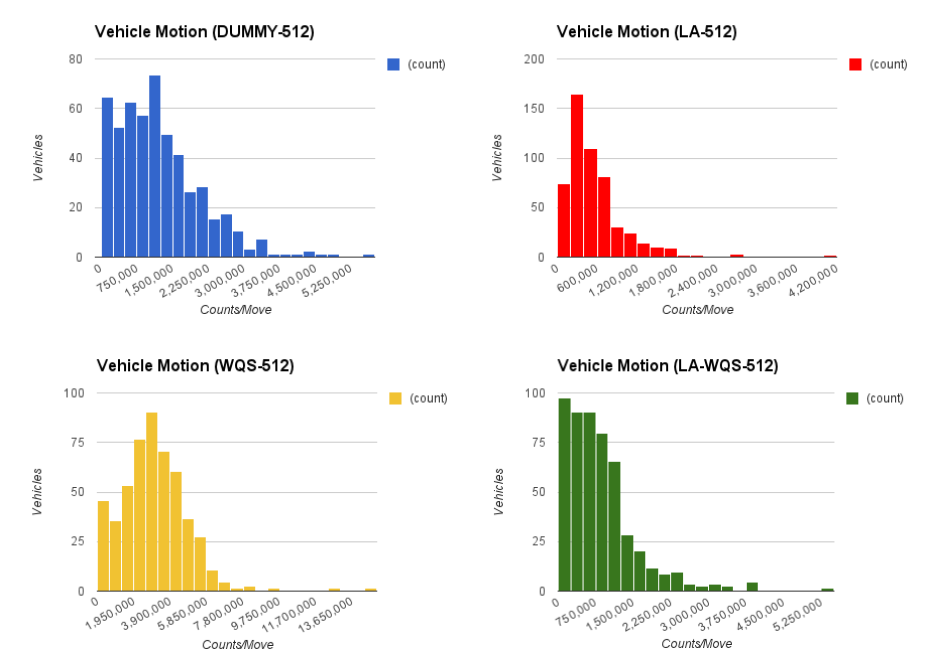
\includegraphics[width=0.5\textwidth]{images/vehicle_motion.png}
	\caption{time spent at each intersection by vehicles. from top-left, clockwise: DUMMY, LA, LA-WQS, WQS}
	\label{vehicle_motion}
\end{figure}

\section{Conclusion}
In this paper, we have presented a simplified framework to model a sophisticated traffic controlling problem, proposed two families of distributed algorithms, and demonstrated their effectiveness in making improvements for both overall traveling time and load-balancing of grid traffic. Our proposed algorithms, LA, WQS, and LA-WQS, all outperforms the benchmark Dummy algorithm under various configurations. We have also shown that with naive definition of queue weights in WQS, the improvements can be limited or even suffer from starvation. 

In conclusion, our main contribution from this work is to demonstrate the effectiveness of two intuitive solutions in online traffic management. One is the advancement of knowledge (Look-Ahead), and the other is an adaptive state machine (WeightedQ-Switcher). With the rise of ubiquitous networks and affordable cloud computing, we believe that these concepts can greatly improve our daily commutes in the near future.

\section{Future Improvements}

To conserve message complexity and computation overhead, each intersection process can easily cache the queue weights of neighboring servers and updates the data under the publisher/subscriber paradigm \cite{pub sub}. On the other hand, we can have more sophisticated state architecture and GridWorld modeling, and test our simulation with real-world traffic data to address potential concerns in practice. Finally, we can improve Look-Ahead by increasing the number of hops to cascade the common knowledge in the system.

\section{Acknowledgements}

We would like to thank Dr. Garg and The University of Texas at Austin for giving us guidance and opportunity to work on this project.

\begin{thebibliography}{1}

\bibitem{pubsub}
Rajkumar, Ragunathan, Michael Gagliardi, and Lui Sha. "The real-time publisher/subscriber inter-process communication model for distributed real-time systems: design and implementation." Real-Time Technology and Applications Symposium, 1995. Proceedings. IEEE, 1995.

\bibitem{commuting_time}
http://project.wnyc.org/commute-times-us/embed.html

\bibitem{commuting_expense}
http://thinkprogress.org/economy/2013/02/05/1540981/commuters-billions-hours-traffic

\bibitem{dijkstra}
Johnson, Donald B. "A note on Dijkstra's shortest path algorithm." Journal of the ACM (JACM) 20.3 (1973): 385-388.

\end{thebibliography}
\end{document}


